\section{Result and Analysis}
\subsection{Parameters}
\begin{table}[h]
    \centering
    \renewcommand{\arraystretch}{1.5} %
    \begin{tabular}{|c|c|}
        \hline
        \textbf{Parameters} & \textbf{Value} \\
        \hline
        \textbf{Total Datasets} & 7  \\
        \hline
        \textbf{Total images} & 446K  \\
        \hline
        \textbf{Trained images (real and fake)} & 203K , 203K \\
        \hline
        \textbf{Tested images (real and fake)} & 10K , 10K \\
        \hline
        \textbf{Validation (real and fake)} & 10K , 10K \\
        \hline
        \textbf{Balanced} &  True\\
        \hline
        \textbf{Epochs} &  10\\
        \hline
        \textbf{Batch Size} &  32\\
        \hline
        \textbf{Image Size} &  256 x 256\\
        \hline
        \textbf{Channels} &  3\\
        \hline
        \textbf{Patches} & 16 x 16\\
        \hline
        \textbf{Encoder Hidden Layers} & 12\\
        \hline
        \textbf{Encoder Layers Dimension} & 768\\
        \hline
        \textbf{MLP size} & 3072\\
        \hline
        \textbf{ Number of Attention Heads } & 12\\
        \hline
        \textbf{Loss Function} & Cross-Entropy Loss \\
        \hline
        \textbf{Normalization} & Layer Normalization \\
        \hline
        \textbf{Activation Function} & GeLU \\
        \hline
        \textbf{Dropout Rate } & 0.2  \\
        \hline
        \textbf{Pooling Strategy } & CLS Token \\
        \hline
    \end{tabular}
    \caption{Model Parameters}
    \label{tab:model-parameters}
\end{table}
\subsection{Evaluation}
The performance of our model is associated with various metrics such as: 
\begin{enumerate}
    \item \textbf{Accuracy:}
           The accuracy metric measures how correctly the model predicts instances by calculating the ratio of correctly classified instances to the total samples.
           \[ Accuracy = \frac{TP + TN}{TP + FP + TN + FN} \]
    
    \item \textbf{Precision:}
           Precision assesses the model's ability to identify positive samples among the actual positives, calculated as the ratio of true positives to the sum of true positives and false positives.

           \[ Precision = \frac{TP}{TP + FP} \]
    
    \item \textbf{Recall (Sensitivity or True Positive Rate):}
           Recall measures the model's ability to precisely identify positive samples from the actual positives, calculated as the ratio of true positives to the sum of true positives and false negatives.

           \[ Recall = \frac{TP}{TP + FN} \]
       
    
    \item \textbf{F1 Score:}
       
           The F1 score, a balance between precision and recall, is advantageous in scenarios with unequal class distribution or equal emphasis on both types of errors. It ranges between 0 and 1, with peak performance at 1.

           \[ F1 = \frac{2 \cdot Precision \cdot Recall}{Precision + Recall} \]
      
    \end{enumerate}
    
\subsection{Work Completed}
\subsubsection{User Interface of Mobile application}
% \begin{itemize}
%     \item a
% \end{itemize}
\subsubsection{Backend}
% \begin{itemize}
   
% \end{itemize}
\subsubsection{Machine Learning Model}
% \begin{itemize}
    
% \end{itemize}

\subsection{Work Remaining}
% \begin{itemize}
    
% \end{itemize}

\subsection{UI of Project}
We have used Flutter and Django to develop the mobile application in which we prepared a
UI with user authentication, login page and home page where we can upload images to be classified as fake and real.\\

\begin{figure}[ht]
    \centering
    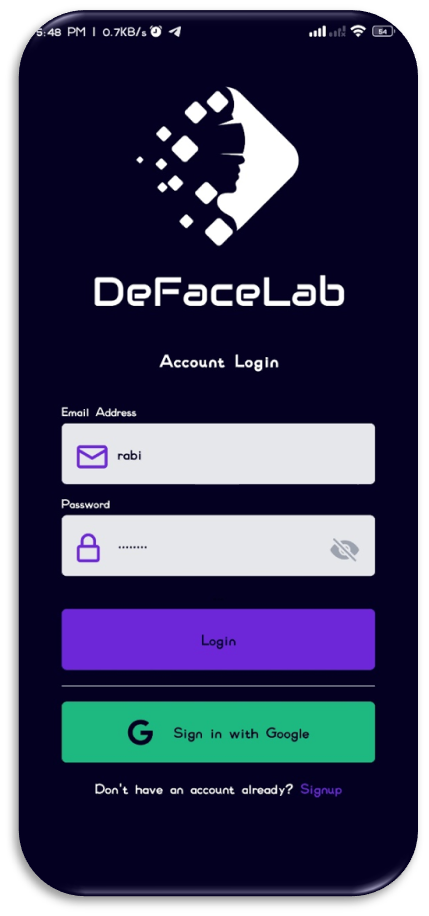
\includegraphics[ height =5in ]{img/loginv3.png}
    \caption{\textit{Login Page }}
\end{figure}

\begin{figure}[ht]
    \centering
    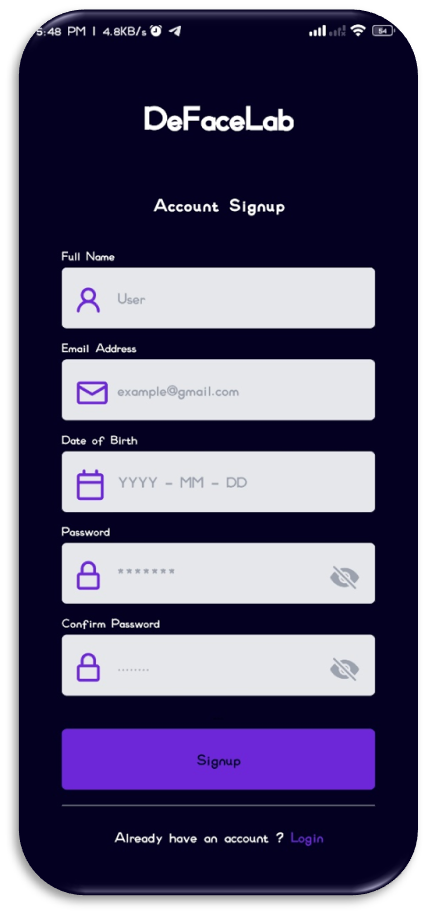
\includegraphics[height= 5in]{img/signup.png}
    \caption{\textit{Sign-up form}}
\end{figure}
\begin{figure}[ht]
    \centering
    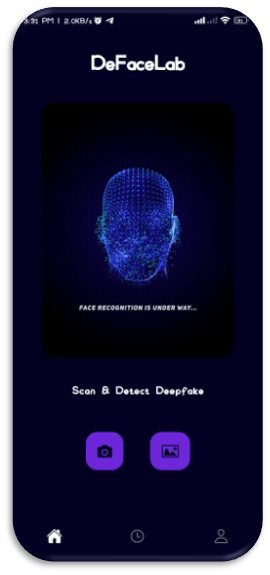
\includegraphics[height =5in ]{img/Homepage.png}
    \caption{\textit{Home Page}}
\end{figure}

\begin{figure}[ht]
    \centering
    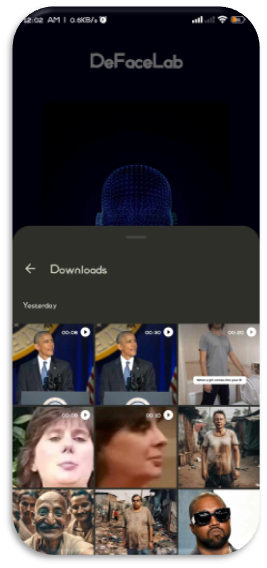
\includegraphics[height =5in ]{img/uploaderv3.png}
    \caption{\textit{Uploader}}
\end{figure}

\begin{figure}[ht]
    \centering
    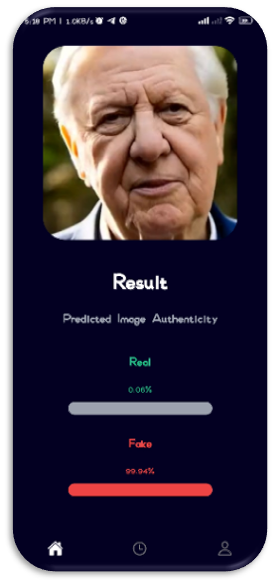
\includegraphics[height= 5in]{img/Results.png}
    \caption{\textit{Result}}
\end{figure}

\begin{figure}[ht]
    \centering
    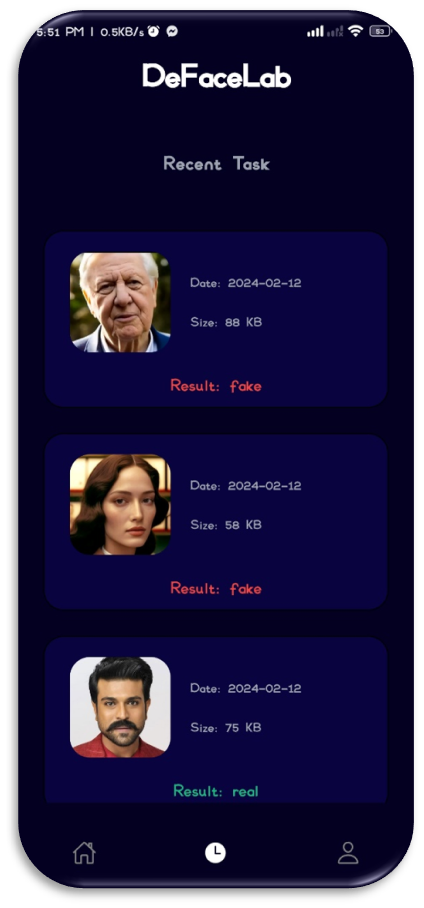
\includegraphics[height= 5in]{img/Historyv2.png}
    \caption{\textit{History page}}
\end{figure}


\begin{figure}[ht]
    \centering
    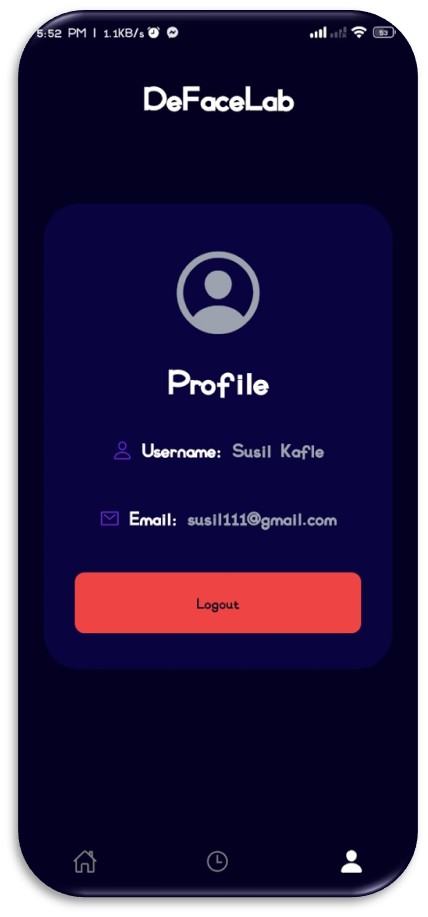
\includegraphics[height= 5in]{img/profilev2.png}
    \caption{\textit{Profile page}}
\end{figure}